\documentclass{beamer}
\setbeamerfont{subsection in toc}{size=\footnotesize}
%\setbeameroption{show notes on second screen=left} %enable for notes
\usepackage{graphicx}
\usepackage{xcolor}
\usepackage{listings}
\usepackage{hyperref}
\lstset{language=python,frame=single}
\usepackage{verbatim}
\usepackage[longnamesfirst]{natbib}
\usepackage{subcaption}
\usepackage{amsmath}
\usepackage{bm}
\usepackage{relsize}
\usepackage{appendixnumberbeamer}
\usepackage{xparse}
\usepackage{multimedia}
\usepackage{xcolor}
\usepackage[normalem]{ulem}
\usepackage{hyperref}
\usepackage{pdfpc-commands}
\usepackage{tikz}
\usetikzlibrary{matrix,backgrounds}
\usetikzlibrary{positioning}
\usetikzlibrary{shapes,arrows}
\usetikzlibrary{decorations.pathreplacing, calligraphy}

\captionsetup[subfigure]{labelformat=empty}

\tikzset{onslide/.code args={<#1>#2}{%
  \only<#1>{\pgfkeysalso{#2}} 
}}

\tikzstyle{block} = [rectangle, draw, thick, align=center, rounded corners]
\tikzstyle{boundingbox} = [thick, lightgray]
\tikzstyle{dashblock} = [rectangle, draw, thick, align=center, dashed]
\tikzstyle{conc} = [ellipse, draw, thick, dashed, align=center]
\tikzstyle{netnode} = [circle, draw, very thick, inner sep=0pt, minimum size=0.5cm]
\tikzstyle{relunode} = [rectangle, draw, very thick, inner sep=0pt, minimum size=0.5cm]
\tikzstyle{line} = [draw, very thick, -latex', -]
\tikzstyle{arrow} = [draw, ->, very thick]

\def\checkmark{\tikz\fill[scale=0.4](0,.35) -- (.25,0) -- (1,.7) -- (.25,.15) -- cycle;}
\def\bigcheckmark{\tikz\fill[scale=0.66](0,.35) -- (.25,0) -- (1,.7) -- (.25,.15) -- cycle;}

\definecolor{bpurp}{HTML}{984ea3}
\definecolor{bblue}{HTML}{377eb8}
\definecolor{bgreen}{HTML}{4daf4a}
\definecolor{borange}{HTML}{ff7f00}
\definecolor{bred}{HTML}{e41a1c}

\usetheme[numbering=none]{metropolis}

\begin{document}

\title{A computational framework for learning and transforming task representations}
\author{Andrew Lampinen}
\date{May 12th, 2020}
\frame{\titlepage}

%{
%\setbeamercolor{background canvas}{bg=white}
%\begin{frame}
%\centering
%\inlineMovie{figures/zooming_in.avi}{figures/zooming_in.png}{width=\textheight, height=\textheight}
%\end{frame}
%}

\begin{frame}%{Broader context}
\begin{columns}
\begin{column}{\dimexpr\paperwidth-1em}
\centering
\begin{tikzpicture}[auto]
\node at (-4.5, 2) {\includegraphics[width=3cm]{figures/papers/paper0.png}};
\node at (-1.5, 2) {\includegraphics[width=3cm]{figures/papers/paper1.png}};
\node at (1.5, 2) {\includegraphics[width=3cm]{figures/papers/paper2.png}};
\node at (4.5, 2) {\includegraphics[width=3cm]{figures/papers/paper3.png}};

\node at (-4.5, -2) {\includegraphics[width=3cm]{figures/papers/paper4.png}};
\node at (-1.5, -2) {\includegraphics[width=3cm]{figures/papers/paper5.png}};
\node at (1.5, -2) {\includegraphics[width=3cm]{figures/papers/paper6.png}};
\node at (4.5, -2) {\includegraphics[width=3cm]{figures/papers/paper7.png}};

\uncover<2->{
\draw[bred, line width=1em] (-6, -3.5) to (6, 3.5);
\draw[bred, line width=1em] (-6, 3.5) to (6, -3.5);
}
\end{tikzpicture}
\end{column}
\end{columns}
\end{frame}

\begin{frame}<1-2>[label=pokermotivation]
\frametitle<1-2>{Human cognition is flexible -- we can adapt on our first try}
\frametitle<3-4>{Adaptation as task transformation}
\frametitle<5>{Switching to opposite rewards is challenging}
\centering
\only<1,5>{
\includegraphics[width=\textwidth]{figures/poker.png}
}
\only<2>{
\includegraphics[width=\textwidth]{figures/old_people_looking_0.png}
}
\only<3>{
\includegraphics[width=\textwidth]{figures/poker_adaptation_0.png}
}
\only<4>{
\includegraphics[width=\textwidth]{figures/poker_adaptation_1.png}
}
\end{frame}
%% Don't forget to say starting point!!!

\begin{frame}{While deep learning is effective at individual tasks...}
\centering
\begin{tikzpicture}[remember picture]
\node at (-1.5, 2) {\includegraphics[width=0.66\textwidth]{figures/imagenet.jpg}};
\node at (-3, -1.5) {\includegraphics[width=0.3\textwidth]{figures/dqn_atari_human.jpg}};
\node at (3.8, 2) {\includegraphics[width=0.3\textwidth]{figures/alphago.jpg}};
\node at (2.25, -1.5) {\includegraphics[width=0.66\textwidth]{figures/poker_superhuman.png}};
\end{tikzpicture}
\end{frame}

\begin{frame}{... it is often criticized for its inflexibility}
\includegraphics[width=\textwidth]{figures/deep_learning_flexibility_critiques.png}
{\scriptsize (Lake, Ullman, Tenenbaum \& Gershman, 2016; Marcus, 2018; Hao, 2020)}
\end{frame}

\begin{frame}{In particular, is deep learning a good cognitive model?}
\phantom{}
{
\centering
\includegraphics[width=0.8\textwidth]{figures/brenden.png}\\
}
{\scriptsize (Lake, Ullman, Tenenbaum \& Gershman, 2016; not exact quotes.)}
\end{frame}

\begin{frame}[standout]
Could deep learning models reuse their knowledge more flexibly, without retraining?
\end{frame}

\againframe<3-4>{pokermotivation}

\begin{frame}[standout]
Goal: a deep-learning framework that can transform task representations to adapt.
\end{frame}

\begin{frame}{Prior work on flexible deep learning models}
I'll discuss the relationship between my work and some of these as I go along.
\begin{itemize}
    \item Meta-learning (learning to learn).
    \item Zero-shot task performance from language.
    \item Model-based methods. 
\end{itemize}
(Happy to address other related work in the Q + A!)
\end{frame}

\section{Meta-mapping}

\begin{frame}{Tasks as functions/mappings}
\begin{columns}
\begin{column}{0.5\textwidth}
It's useful to think of tasks or behaviors as functions mapping input to output:
\begin{itemize}
    \item Poker hand \(\rightarrow\) bet
    \item Chess position \(\rightarrow\) move
    \item Image \(\rightarrow\) classification
\end{itemize}
Standard deep learning tries to infer this mapping from lots of examples, meta-learning from fewer. 
\end{column}

\begin{column}{0.5\textwidth}
\includegraphics[width=\textwidth]{figures/poker_function.png}
\end{column}
\end{columns}
\end{frame}

\begin{frame}{Generalizing tasks from examples}
\centering
\includegraphics[height=0.8\textheight]{figures/poker_from_examples.png}
\end{frame}

\begin{frame}[standout]
Tasks \(\bm =\) mappings from inputs to outputs.\\[1em] 
\uncover<2>{
Task mappings can be inferred from examples.
}
\end{frame}

%% TODO: Maybe cut
%\begin{frame}{Meta-learning}
%\begin{columns}
%\begin{column}{0.5\textwidth}
%
%\begin{itemize}[<+->]
%    \item Lots of recent research on meta-learning -- learning to learn.
%    \item If you have learned a lot of card games, you should be able to pick up a new one from a few examples.
%    \item Then apply this knowledge to play the game with probe hands you weren't taught. 
%    \item But, again, how could we play a variation of the game without examples? 
%\end{itemize}
%\end{column}
%
%\begin{column}{0.5\textwidth}
%\includegraphics[width=\textwidth]{figures/poker_function_2.png}
%\end{column}
%\end{columns}
%\end{frame}

\begin{frame}{Altering the task = adapting the mapping}
\only<1>{
\includegraphics[width=\textwidth]{figures/poker_adaptation_1.png}
}
\only<2>{
\includegraphics[width=\textwidth]{figures/poker_adaptation_mappings.png}
}
\end{frame}

%\begin{frame}[standout]
%We want to model how we can transform the task mapping.
%\end{frame}

\begin{frame}{Meta-mappings}
How do we adapt a task-mapping?
\begin{itemize}
\item We propose \textbf{meta-mappings}, higher-order mappings which transform task mappings into other task mappings.
\end{itemize}
\includegraphics[width=\textwidth]{figures/meta_mapping_poker.png}
\end{frame}

\begin{frame}[standout]
Transforming the task mapping \(=\) adapting. \\[1em]
Meta-mappings are higher-order mappings that transform task mappings.
\end{frame}

\begin{frame}{Could we generalize meta-mappings from examples?}
\centering
\includegraphics[height=0.8\textheight]{figures/losing_from_examples.png}
\end{frame}

\begin{frame}<-3>[label=basic_metamapping_analogy]
\frametitle{Meta-mappings are analogous to basic tasks}
\begin{columns}
\begin{column}{0.5\textwidth}
\vspace{2em}
\includegraphics[width=\textwidth]{figures/poker_function.png}
\end{column}
\begin{column}{0.5\textwidth}
\vspace{2em}
\includegraphics[width=\textwidth]{figures/try_to_lose_function.png}
\end{column}
\end{columns}
\only<-3>{
\begin{itemize}[<+->]
\item Both are just functions (they just have different types of inputs and outputs).
\item This means we can apply all the usual deep learning tricks to meta-mappings.
\item ... Assuming we have a way to represent the basic tasks for input to (and output from) the meta-mappings. 
\end{itemize}
}
\end{frame}

\begin{frame}[standout]
There is a functional analogy between basic tasks and meta-mappings. \\[1em]
But we need task representations to use it. 
\end{frame}

\section{An architecture for representing and transforming tasks}

\begin{frame}{Architecture preview}
Our goal is to implement:
\begin{itemize}
\item A way of representing tasks as mappings.
\item A way of representing those tasks/mappings as vectors.
\item A way of learning to transform those task-vectors to perform meta-mappings.
\end{itemize}
This will allow the architecture to perform new tasks without data, by their relationship to prior tasks.
\end{frame}

\begin{frame}<2>{Task-specific computations are low-dimensional and abstract}
\begin{tikzpicture}[auto]
\node at (-4, 0) (image) {\includegraphics[width=2cm]{figures/straight_flush_hand.jpg}};


%% input

\node[netnode] at (-2.25, -1.5) (i00) {};
\node[netnode] at (-2.25, -0.75) (i01) {};
\node[netnode] at (-2.25, 0) (i02) {};
\node[netnode] at (-2.25, 0.75) (i03) {};
\node[netnode] at (-2.25, 1.5) (i04) {};

\path [line] ([xshift=-3]image.east) to (i00);
\path [line] ([xshift=-3]image.east) to (i01);
\path [line] ([xshift=-3]image.east) to (i02);
\path [line] ([xshift=-3]image.east) to (i03);
\path [line] ([xshift=-3]image.east) to (i04);

\node[netnode] at (-1, -1.5) (i10) {};
\node[netnode] at (-1, -0.75) (i11) {};
\node[netnode] at (-1, 0) (i12) {};
\node[netnode] at (-1, 0.75) (i13) {};
\node[netnode] at (-1, 1.5) (i14) {};

\path [line] (i00) to (i10);
\path [line] (i00) to (i11);
\path [line] (i00) to (i12);
\path [line] (i00) to (i13);
\path [line] (i00) to (i14);
\path [line] (i01) to (i10);
\path [line] (i01) to (i11);
\path [line] (i01) to (i12);
\path [line] (i01) to (i13);
\path [line] (i01) to (i14);
\path [line] (i02) to (i10);
\path [line] (i02) to (i11);
\path [line] (i02) to (i12);
\path [line] (i02) to (i13);
\path [line] (i02) to (i14);
\path [line] (i03) to (i10);
\path [line] (i03) to (i11);
\path [line] (i03) to (i12);
\path [line] (i03) to (i13);
\path [line] (i03) to (i14);
\path [line] (i04) to (i10);
\path [line] (i04) to (i11);
\path [line] (i04) to (i12);
\path [line] (i04) to (i13);
\path [line] (i04) to (i14);

%% task specific
\node[netnode] at (0.25, -0.375) (t00) {};
\node[netnode] at (0.25, 0.375) (t01) {};

\path [line] (i10) to (t00);
\path [line] (i10) to (t01);
\path [line] (i11) to (t00);
\path [line] (i11) to (t01);
\path [line] (i12) to (t00);
\path [line] (i12) to (t01);
\path [line] (i13) to (t00);
\path [line] (i13) to (t01);
\path [line] (i14) to (t00);
\path [line] (i14) to (t01);

\node[netnode] at (1.5, -0.375) (t10) {};
\node[netnode] at (1.5, 0.375) (t11) {};

\path [line] (t00) to (t10);
\path [line] (t00) to (t11);
\path [line] (t01) to (t10);
\path [line] (t01) to (t11);

%% output

\node[netnode] at (2.75, -1.5) (o00) {};
\node[netnode] at (2.75, -0.75) (o01) {};
\node[netnode] at (2.75, 0) (o02) {};
\node[netnode] at (2.75, 0.75) (o03) {};
\node[netnode] at (2.75, 1.5) (o04) {};

\path [line] (t10) to (o00);
\path [line] (t11) to (o00);
\path [line] (t10) to (o01);
\path [line] (t11) to (o01);
\path [line] (t10) to (o02);
\path [line] (t11) to (o02);
\path [line] (t10) to (o03);
\path [line] (t11) to (o03);
\path [line] (t10) to (o04);
\path [line] (t11) to (o04);

\node[netnode] at (4, -1.5) (o10) {};
\node[netnode] at (4, -0.75) (o11) {};
\node[netnode] at (4, 0) (o12) {};
\node[netnode] at (4, 0.75) (o13) {};
\node[netnode] at (4, 1.5) (o14) {};

\path [line] (o00) to (o10);
\path [line] (o00) to (o11);
\path [line] (o00) to (o12);
\path [line] (o00) to (o13);
\path [line] (o00) to (o14);
\path [line] (o01) to (o10);
\path [line] (o01) to (o11);
\path [line] (o01) to (o12);
\path [line] (o01) to (o13);
\path [line] (o01) to (o14);
\path [line] (o02) to (o10);
\path [line] (o02) to (o11);
\path [line] (o02) to (o12);
\path [line] (o02) to (o13);
\path [line] (o02) to (o14);
\path [line] (o03) to (o10);
\path [line] (o03) to (o11);
\path [line] (o03) to (o12);
\path [line] (o03) to (o13);
\path [line] (o03) to (o14);
\path [line] (o04) to (o10);
\path [line] (o04) to (o11);
\path [line] (o04) to (o12);
\path [line] (o04) to (o13);
\path [line] (o04) to (o14);

\node at (5.25, 0) (output) {\textbf{\$\$\$}};
\path [line] (o10) to (output.west);
\path [line] (o11) to (output.west);
\path [line] (o12) to (output.west);
\path [line] (o13) to (output.west);
\path [line] (o14) to (output.west);

%% overlays
\uncover<2->{
\draw[fill=black, opacity=0.2] (-2.9, -3.5) rectangle (-0.25, 2);
\draw[fill=black, opacity=0.2] (2, -3.5) rectangle (4.5, 2);
\draw[fill=bblue, opacity=0.4] (-0.25, -3.5) rectangle (2, 2);
}

%% anotations

\node at (-4, -3) {\textbf{Input}};
\node[text width=2.5cm, align=center] at (-1.625, -3) {\textbf{Shared ``perception''}};
\node[text width=2cm, align=center] at (0.875, -3) {\textbf{Task specific}};
\node[text width=2.5cm, align=center] at (3.375, -3) {\textbf{Shared ``action''}};
\node at (5.25, -3) {\textbf{Output}};


\end{tikzpicture}
\end{frame}

\begin{frame}<-4>[label=homm_basic]
\frametitle<1>{Basic task processing}
\frametitle<2-3>{Adapting to a task}
\frametitle<4>{Constructing a task representation}
\frametitle<5->{Now we can transform the task representation!}
\begin{columns}
\begin{column}{\dimexpr\paperwidth-1em}
\resizebox{\textwidth}{!}{%
\begin{tikzpicture}[auto, every node/.style={execute at begin node=\setlength{\baselineskip}{1.1em}}]
%% a) constructing
\only<4->{
\begin{scope}[shift={(0.4, 0)}]
\draw[boundingbox, draw=gray, fill=white] (-8.5, -2.5) rectangle (-2, 2.5);

%% from language
%\node[gray] at (-7, -0.4) {Instructions};
%\node at (-7, -1.25) (language) {``Play poker.''};
%
%\node[gray, text width=2cm, align=center] at (-4.1, -0.4) {Language network};
%\node[block] at (-4.1, -1.25) (languagenet) {\(\mathcal{L}\)};
%\path[arrow] (language.east) -- ([xshift=-3]languagenet.west);
%
%\node[bpurp, text width=2cm] at (-2, -1.25) (languagetaskrep) {\(z_{poker}\)};
%\path[arrow] ([xshift=3]languagenet.east) -- (languagetaskrep.west);


%% from examples

\node[gray, text width=2.5cm, align=center] at (-7, 2) {Task examples (encoded)};
\node at (-7, 1.1) (examples) {
\(\left\{
\begin{matrix}
({\color{bgreen}z_{hand_{1}}}, {\color{bgreen}z_{bet_{1}}})\\
$\vdots$
\end{matrix}\right\}\)};

\node[gray, text width=2cm, align=center] at (-4.1, 2) {Example network};
\node[block] at (-4.1, 1.1) (examplenet) {\(\mathcal{E}\)};
\path[arrow] (examples.east) -- ([xshift=-3]examplenet.west);

\node[bpurp, text width=2cm] at (-2, 1.1) (examplestaskrep) {\(z_{poker}\)};
\path[arrow] ([xshift=3]examplenet.east) -- (examplestaskrep.west);
\end{scope}
}
%% b) performing
\draw[boundingbox, draw=gray, fill=white] (-1.5, -2.5) rectangle (8, 2.5);
\only<2->{
\node[bpurp] at (-0.75, 1.1) (taskrep) {\(z_{poker}\)};

\node[gray, text width=2cm, align=center] at (0.75, 2) {Hyper network};
\node[block] at (0.75, 1.1) (hypernet) {\(\mathcal{H}\)};
\path[arrow] (taskrep.east) -- ([xshift=-3]hypernet.west);
}

\node[text width=0.5cm] at (-0.85, -1.25) (inputs) {\includegraphics[width=0.5cm]{figures/2_of_spades.png}\\\includegraphics[width=0.5cm]{figures/4_of_hearts.png}};

\node[gray, text width=2cm, align=center] at (0.6, -2) {Perception network};
\node[block] at (0.6, -1.25) (perceptionnet) {\(\mathcal{P}\)};
\path[arrow] (inputs.east) -- ([xshift=-3]perceptionnet.west);

\node[bgreen] at (2.05, -1.25) (handrep) {\(z_{hand}\)};
\path[arrow] ([xshift=3]perceptionnet.east) -- (handrep.west);

\node[bblue, block, dashed] at (3.5, -1.25) (tasknet) {\(\mathcal{T}\)};
\node[bblue, text width=1.5cm, align=center] at (3.5, -2) {Task network};
\path[arrow] (handrep.east) -- ([xshift=-3]tasknet.west);
\only<2->{
\path[arrow, out=0, in=90] ([xshift=3]hypernet.east) to ([yshift=3]tasknet.north);
}

\node[bgreen] at (4.85, -1.25) (betrep) {\(z_{bet}\)};
\path[arrow] ([xshift=3]tasknet.east) -- (betrep.west);

\node[gray, text width=2cm, align=center] at (6.2, -2) {Action network};
\node[block] at (6.2, -1.25) (actionnet) {\(\mathcal{A}\)};
\path[arrow] (betrep.east) -- ([xshift=-3]actionnet.west);

\node at (7.4, -1.25) (output) {\bf \$};
\path[arrow] ([xshift=3]actionnet.east) -- (output.west);

%%% d subpanel) task network
\only<3>{
\draw[boundingbox, draw=gray, fill=white] (4.25, 0) rectangle (8, 2.5);
\node[gray] at (6.15, 2.25) {\small \(\mathcal{H}\) adapts weights in \(\mathcal{T}\)};
\begin{scope}[scale=0.9, shift={(0.5, 0.25)}, every node/.append style={transform shape}]
\node at (4.45, 1.45) (pseudohyper) {};

\node[bblue, text width=1.25 cm] at (5, 1.65) (Wprime) {\scriptsize \(W^{\mathcal{H}}, b^{\mathcal{H}}\)};
\node[bblue] at (6, 0.25) (W0) {\scriptsize Default \(W^{0}, b^{0}\)};
\node[netnode, bblue, thick] at (4.75, 0.5) (tnode1) {I};

\node[netnode, bblue, thick] at (7.35, 0.5) (tnode2) {O};
\node[bblue] at (7.2, 1.3) {\scriptsize\(O\!=\!(W^{0}\!+\!W^{\mathcal{H}})I\)};
\node[bblue] at (7.2, 1.0) {\scriptsize\(+(b^{0}\!+\!b^{\mathcal{H}})\)};

\path[arrow, bblue, out=0, in=90] (pseudohyper) to ([yshift=10]W0);
\path[arrow, bblue, dashed] (tnode1) to (tnode2);
\end{scope}

%% connecting to subpanel

\path[draw, gray, thick] (3.75, -0.95) to (4.25, 2.5);
\path[draw, gray, thick] (3.75, -0.95) to (8, 0);
}

\uncover<5->{
%\draw [red, line width=0.25em] (-0.75, 1.1) circle (0.5);
\draw [red, line width=0.25em] (-2.2, 1.1) circle (0.5);
}
\end{tikzpicture}}
\end{column}
\end{columns}
\end{frame}

\begin{frame}[standout]
Our architecture generates task representations from examples, which it uses to modulate a network which performs the task. % shorten this
\end{frame}

\againframe<5>{homm_basic}

\begin{frame}<1>[label=homm_arch]
\frametitle<1>{Meta-mapping as transforming task representations}
\frametitle<2-3>{So we can use the same approach and networks!}
\frametitle<4,7>{A reminder of the approach}
\frametitle<5>{Language-based approach}
\frametitle<6>{Language-based meta-mapping}
%\frametitle<4>{Language-based meta-mapping}
\begin{columns}
\begin{column}{\dimexpr\paperwidth-10pt}
\centering
\only<3->{
\resizebox{\dimexpr\textwidth-1pt}{!}{%
\begin{tikzpicture}[auto, every node/.style={execute at begin node=\setlength{\baselineskip}{1.1em}}]
\begin{scope}[shift={(0.4, 0)}]
%% a) constructing
\draw[boundingbox, draw=gray, fill=white] (-8.5, -2.5) rectangle (-2, 2.5);

%% from language
\only<5-6>{
\node[gray] at (-7, -0.4) {Instructions};
\node at (-7, -1.25) (language) {\only<-5>{``Play poker.''}\only<6>{``Red \& square.''}};

\node[gray, text width=2cm, align=center] at (-4.1, -0.4) {Language network};
\node[block] at (-4.1, -1.25) (languagenet) {\(\mathcal{L}\)}; 
\path[arrow] (language.east) -- ([xshift=-3]languagenet.west);

\node[bpurp, text width=2cm] at (-2, -1.25) (languagetaskrep) {\only<-5>{\(z_{poker}\)}\only<7>{\(z_{task}\)}\only<6>{\(z_{r,sq}\)}}; 
\path[arrow] ([xshift=3]languagenet.east) -- (languagetaskrep.west);
}


%% from examples
\only<-4,7->{

%\only<4>{
%\begin{scope}[shift={(0, 2.5)}]
%}

\node[gray, text width=2.5cm, align=center] at (-7, 2) {Task examples (encoded)};
\node at (-7, 1.1) (examples) {
\(\left\{
\begin{matrix}
\only<1-5>{({\color{bgreen}z_{hand_{1}}}, {\color{bgreen}z_{bet_{1}}})\\}
\only<6->{({\color{bgreen}z_{state}}, {\color{bgreen}z_{(a,r)}})\\}
$\vdots$
\end{matrix}\right\}\)};

%\only<-3, 5-6>{
\node[gray, text width=2cm, align=center] at (-4.1, 2) {Example network};
%}
\node[block] at (-4.1, 1.1) (examplenet) {\(\mathcal{E}\)}; 
\path[arrow] (examples.east) -- ([xshift=-3]examplenet.west);

\node[bpurp, text width=2cm] at (-2, 1.1) (examplestaskrep) {\only<-5>{\(z_{poker}\)}\only<7>{\(z_{task}\)}\only<6>{\(z_{r,sq}\)}}; 
\path[arrow] ([xshift=3]examplenet.east) -- (examplestaskrep.west);
%\only<4>{
%\end{scope}
%}
}

\end{scope}
%% b) performing 
\draw[boundingbox, draw=gray, fill=white] (-1.5, -2.5) rectangle (8.5, 2.5);
\node[bpurp] at (-0.75, 1.1) (taskrep) {\only<-5>{\(z_{poker}\)}\only<7>{\(z_{task}\)}\only<6>{\(z_{r,sq}\)}};

\node[gray, text width=2cm, align=center] at (0.75, 2) {Hyper network};
\node[block] at (0.75, 1.1) (hypernet) {\(\mathcal{H}\)}; 
\path[arrow] (taskrep.east) -- ([xshift=-3]hypernet.west);

\node[text width=0.5cm] at (-0.85, -1.25) (inputs) {
    \only<-5>{\includegraphics[width=0.5cm]{figures/2_of_spades.png}\\\includegraphics[width=0.5cm]{figures/4_of_hearts.png}}
    \only<7>{\includegraphics[width=0.5cm]{../../psych/dissertation/4-extending/figures/pick_up_0.png}}
    \only<6>{\includegraphics[width=0.5cm]{figures/categorization/32_cyan_emptysquare_0.png}}
};

\node[gray, text width=2cm, align=center] at (0.6, -2) {Perception network};
\node[block] at (0.6, -1.25) (perceptionnet) {\(\mathcal{P}\)}; 
\path[arrow] (inputs.east) -- ([xshift=-3]perceptionnet.west);

\node[bgreen] at (2.05, -1.25) (handrep) {\only<-5>{\(z_{hand}\)}\only<7>{\(z_{state}\)}\only<6>{\(z_{im}\)}};
\path[arrow] ([xshift=3]perceptionnet.east) -- (handrep.west);

\node[bblue, block, dashed] at (3.5, -1.25) (tasknet) {\(\mathcal{T}\)}; 
\node[bblue, text width=1.5cm, align=center] at (3.5, -2) {Task network};
\path[arrow] (handrep.east) -- ([xshift=-3]tasknet.west);
\path[arrow, out=0, in=90] ([xshift=3]hypernet.east) to ([yshift=3]tasknet.north);


\node[bgreen] at (4.85, -1.25) (betrep) {\only<-5>{\(z_{bet}\)}\only<7>{\(z_{act}\)}\only<6>{\(z_{cls}\)}};
\path[arrow] ([xshift=3]tasknet.east) -- (betrep.west);

\node[gray, text width=2cm, align=center] at (6.2, -2) {Action network};
\node[block] at (6.2, -1.25) (actionnet) {\(\mathcal{A}\)}; 
\path[arrow] (betrep.east) -- ([xshift=-3]actionnet.west);

\node at (7.4, -1.25) (output) {\bf \only<-5>{\$}\only<6>{0}\only<7>{``\(\uparrow\)''}};
\path[arrow] ([xshift=3]actionnet.east) -- (output.west);
\end{tikzpicture}}}\\%
\resizebox{\textwidth}{!}{%
\begin{tikzpicture}[auto, every node/.style={execute at begin node=\setlength{\baselineskip}{1.1em}}]
\setlength{\baselineskip}{1.2em}
\only<-4,6->{
\only<2->{
\begin{scope}[shift={(0.4, 0)}]
%% a) constructing
\draw[boundingbox, draw=gray, fill=white] (-8.5, -2.5) rectangle (-2, 2.5);

%% from language
\only<5-6>{
\node[gray] at (-6.7, -0.4) {Instructions};
\node at (-6.7, -1.25) (language) {\only<-5>{``Try to lose.''}\only<7>{``Switch.''}\only<6>{``Red\(\mapsto\)blue.''}};

\node[gray, text width=2cm, align=center] at (-4.1, 0.4) {Language network};
\node[block] at (-4.1, -1.25) (languagenet) {\(\mathcal{L}\)}; 
\path[arrow] (language.east) -- ([xshift=-3]languagenet.west);

\node[borange, text width=2cm] at (-2, -1.25) (languagetaskrep) {\only<-5>{\(z_{lose}\)}\only<7>{\(z_{switch}\)}\only<6>{\(z_{r\mapsto b}\)}}; 
\path[arrow] ([xshift=3]languagenet.east) -- (languagetaskrep.west);
}


%% from examples

\only<-4,7>{
\node[gray, text width=3.5cm, align=center] at (-6.7, 2) {Mapping examples (task pairs)};
\node at (-6.7, 1.1) (examples) {
\(\left\{
\begin{matrix}
\only<-4>{({\color{bpurp}z_{hearts}}, {\color{bpurp}z_{lose hearts}})\\}
\only<5->{({\color{bpurp}z_{task}}, {\color{bpurp}z_{swtask}})\\}
$\vdots$
\end{matrix}\right\}\)};

\node[gray, text width=2cm, align=center] at (-4.1, 2) {Example network};
\node[block] at (-4.1, 1.1) (examplenet) {\(\mathcal{E}\)}; 
\path[arrow] ([xshift=-3]examples.east) -- ([xshift=-3]examplenet.west);

\node[borange, text width=2cm] at (-2, 1.1) (examplestaskrep) {\only<-5>{\(z_{lose}\)}\only<7>{\!\(z_{switch}\)}\only<6>{\(z_{r\mapsto b}\)}}; 
\path[arrow] ([xshift=3]examplenet.east) -- (examplestaskrep.west);
}

\end{scope}
}
%% d) performing 
\draw[boundingbox, draw=gray, fill=white] (-1.5, -2.5) rectangle (8.5, 2.5);
\only<2->{
\node[borange] at (-0.75, 1.1) (taskrep) {\only<-5>{\(z_{lose}\)}\only<7>{\(z_{switch}\)}\only<6>{\(z_{r\mapsto b}\)}};

\node[gray, text width=2cm, align=center] at (0.75, 2) {Hyper network};
\node[block] at (0.75, 1.1) (hypernet) {\(\mathcal{H}\)}; 
\path[arrow] (taskrep.east) -- ([xshift=-3]hypernet.west);
}

\node[bpurp] at (1.66, -1.25) (handrep) {\only<-5>{\(z_{poker}\)}\only<7>{\(z_{task}\)}\only<6>{\(z_{r,sq}\)}};

\only<1>{
\node[bblue, block, dashed] at (3.5, -1.25) {??}; 
}
\uncover<1>{
\node at (4, -1.9) {\includegraphics[height=1cm]{figures/wizard.png}};
}
\uncover<2->{
\node[bblue, block, dashed] at (3.5, -1.25) (tasknet) {\(\mathcal{T}\)}; 
}
\path[arrow] (handrep.east) -- ([xshift=-3]tasknet.west);
\only<2->{
\node[bblue, text width=1.5cm, align=center] at (3.5, -2) {Task network};
\path[arrow, out=0, in=90] ([xshift=3]hypernet.east) to ([yshift=3]tasknet.north);
}

\node[bpurp] at (5.5, -1.25) (output) {\only<-5>{\(z_{losepoker}\)}\only<7>{\(z_{switchedtask}\)}\only<6>{\(z_{b,sq}\)}};
\path[arrow] ([xshift=3]tasknet.east) -- (output.west);

%% d subpanel) performing basic from meta-mapped

\draw[boundingbox, draw=gray, fill=white] (4.25, 0) rectangle (8.5, 2.5);
\node[gray] at (6.35, 2.25) {Performing the new task};
\begin{scope}[scale=0.5, shift={(8.5,2.5)}, every node/.append style={transform shape}]

\node[gray, text width=2cm, align=center] at (2, 1.1) {Hyper network};
\node[block, semithick, rounded corners=2] at (2, 0.25) (hypernet2) {\(\mathcal{H}\)}; 

\node[text width=0.5cm] at (0.7, -1.25) (inputs2) {
    \only<-5>{\includegraphics[width=0.5cm]{figures/2_of_spades.png}\\\includegraphics[width=0.5cm]{figures/4_of_hearts.png}}
    \only<7>{\includegraphics[width=0.5cm]{../../psych/dissertation/4-extending/figures/pick_up_0.png}}
    \only<6>{\includegraphics[width=0.5cm]{figures/categorization/32_cyan_emptysquare_0.png}}
};

\node[gray, text width=2cm, align=center] at (1.9, -2) {Perception network};
\node[block, semithick, rounded corners=2] at (1.9, -1.25) (perceptionnet2) {\(\mathcal{P}\)}; 
\path[arrow, semithick] (inputs2.east) -- ([xshift=-3]perceptionnet2.west);

\node[bgreen] at (3.2, -1.25) (handrep2) {\only<-5>{\(z_{hand}\)}\only<7>{\(z_{state}\)}\only<6>{\(z_{im}\)}};
\path[arrow, semithick] ([xshift=3]perceptionnet2.east) -- (handrep2.west);

\node[bblue, block, semithick, rounded corners=2, dash pattern=on 2pt off 2pt] at (4.5, -1.25) (tasknet2) {\(\mathcal{T}\)}; 
\node[bblue, text width=1.5cm, align=center] at (4.5, -2) {Task network};
\path[arrow, semithick] (handrep2.east) -- ([xshift=-3]tasknet2.west);
\path[arrow, semithick, out=0, in=90] ([xshift=3]hypernet2.east) to ([yshift=3]tasknet2.north);

\node[bgreen] at (5.65, -1.25) (betrep2) {\only<-5>{\(z_{bet}\)}\only<7>{\(z_{act}\)}\only<6>{\(z_{cls}\)}};
\path[arrow, semithick] ([xshift=3]tasknet2.east) -- (betrep2.west);

\node[gray, text width=2cm, align=center] at (6.8, -2) {Action network};
\node[block, semithick, rounded corners=2] at (6.8, -1.25) (actionnet2) {\(\mathcal{A}\)}; 
\path[arrow, semithick] (betrep2.east) -- ([xshift=-3]actionnet2.west);

\node at (7.8, -1.25) (output2) {\bf \only<-5>{\$}\only<6>{0}\only<7>{``\(\uparrow\)''}};
\path[arrow] ([xshift=3]actionnet2.east) -- (output2.west);
\end{scope}

%% connecting to subpanel

\node[inner sep=0, outer sep=0] at (6.8, -0.8) (c1) {};
\node[inner sep=0, outer sep=0] at (4.5, -0.3) (c2) {};
\node[inner sep=0, outer sep=0] at (4, 0.5) (c3) {};
\path[draw, gray, very thick, out=0, in=-90, dash pattern=on 2pt off 2pt] (output.east) to (c1);
\path[draw, gray, very thick, out=90, in=0, dash pattern=on 2pt off 2pt] (c1) to (c2);
\path[draw, gray, very thick, out=180, in=-90, dash pattern=on 2pt off 2pt] (c2) to (c3);
\path[arrow, gray, very thick, out=90, in=180, dash pattern=on 2pt off 2pt] (c3) to ([xshift=-3]hypernet2.west);
}
\end{tikzpicture}}
\end{column}
\end{columns}
\end{frame}


\againframe<4>{basic_metamapping_analogy}

\againframe<2-3>{homm_arch}

\begin{frame}[standout]
We can use the same approaches and networks for both basic tasks and meta-mappings.
\end{frame}

%% TODO: reinsert?
\begin{frame}{Meta-mapping summary}
\begin{itemize}
\item Basic tasks are mappings from inputs to outputs (e.g. poker hands to bets), which can be inferred from examples.
\item We represent the task-specific computations as relatively simple transformations, parameterized from a task representation. The rest of input and output is shared across tasks.
\item One type of flexibility is systematically altering these tasks (e.g. trying to bet on losing hands instead of winning ones).
\item This can be seen as a \textbf{meta-mapping}, that is, a mapping which takes tasks as input and produces tasks as output (e.g. maps try-to-win-at-poker to try-to-lose-at-poker).
\item We implement the meta-mapping function as a transformation of task embeddings.
\item This mapping can be parsimoniously inferred and implemented using exactly the same networks as the basic tasks.
\end{itemize}
\end{frame}

\section{Explorations}

%\begin{frame}{Explorations overview}
%This same approach can be used in many different settings: 
%\begin{table}
%\center
%\begin{tabular}{|c|c|c|}
%\hline
%Experiment & Type & Cognitive motivation \\
%\hline
%\color{lightgray} Polynomials & \color{lightgray} Regression & \color{lightgray} Proof of concept \\
%Card games & Regression & Adapting strategies \\
%2D worlds & RL & Adapting behaviors \\
%Categories & Classification & Adapting concepts \\
%\hline
%\end{tabular}
%\end{table}
%\end{frame}
%
\againframe<5>{pokermotivation}

\begin{frame}{Simple card games}

\begin{itemize}
\item Constructed 5 two-card games (analogous to poker, blackjack, etc.)
\item With 8 variations of each, including ``try-to-lose'' variations
\item Taught the model winning variations of poker, and winning and losing variations of other games 
\item Can it infer losing at poker?
\end{itemize}
%\begin{columns}
%\begin{column}{0.5\textwidth}
%Five games:
%\begin{itemize}
%\item \textbf{High card:} Highest wins.
%\item \textbf{Pairs:} Pairs are valuable. 
%\item \textbf{Match:} Closest to matching cards win. 
%\item \textbf{Blackjack:} Value increases to a threshold, then switches to negative. 
%\item \textbf{Straight flush:} Adjacent same suit numbers are best, then adjacent different. 
%\end{itemize}
%\end{column}
%
%\begin{column}{0.5\textwidth}
%Three binary attributes:
%\begin{itemize}
%\item \textbf{Losers:} Try to lose instead of winning! Reverses the ranking of hands.
%\item \textbf{Suits rule:} Suits are more important than values. 
%\item \textbf{Switch suit:} Switches which of the suits is more valuable.
%\end{itemize}
%\vspace{3.2em}
%\end{column}
%\end{columns}
%\vspace{1em}
%\textbf{= 40 total, held out all four ``straight flush'' losing versions}
\end{frame}

\againframe<4>{homm_arch}

\begin{frame}
\frametitle<1>{Possible results}
\frametitle<2->{Meta-mapping results}
\only<1>{
\includegraphics[height=0.8\textheight]{figures/cards_patterns_interpretation.png}
}
\only<2>{
\includegraphics[height=0.8\textheight]{../../psych/dissertation/3-human-adaptation/figures/adaptation_HoMM_only.png}
\begin{tikzpicture}[overlay]
\fill[white] (-3, 2) rectangle (-0.2, 5); 
\end{tikzpicture}
}
\end{frame}

\begin{frame}[standout]
Meta-mapping adapts well! But how well?
\end{frame}

\againframe<5>{homm_arch}
%TODO: new language intro

\begin{frame}<1>[label=cards_results]
\frametitle<1>{MM vs. language}
\frametitle<2->{MM vs. humans}
\only<1>{ 
\includegraphics[height=0.8\textheight]{../../psych/dissertation/3-human-adaptation/figures/adaptation_HoMM_langauge.png}
\begin{tikzpicture}[overlay]
\fill[white] (-3, 3.5) rectangle (-0.2, 4); 
\end{tikzpicture}
}
\only<2>{
\includegraphics[height=0.8\textheight]{../../psych/dissertation/3-human-adaptation/figures/human_adaptation_vs_HoMM.png}
Note: Human variability is mostly internal, not due to experiment.
}
\only<3>{
\includegraphics[height=0.8\textheight]{../../psych/dissertation/3-human-adaptation/figures/change_scores.png}
Note: this analysis is biased against models because of ceiling.
}
\end{frame}

\begin{frame}{Human comparison}
\begin{columns}
\begin{column}{0.5\textwidth}
\begin{itemize}
\item On mTurk, taught 40 subjects this card game.
\item Instructions + hand comparisons to illustrate rules.
\item 32 practice trials where they saw outcome.
\item 24 testing trials without outcome.
\item Told to lose, 24 more testing trials without outcome.
\end{itemize}
\end{column}

\begin{column}{0.5\textwidth}
\vspace{1em}
\includegraphics[width=\textwidth]{../../psych/dissertation/3-human-adaptation/figures/pre_bet_screenshot.png}
\includegraphics[width=\textwidth]{../../psych/dissertation/3-human-adaptation/figures/post_bet_screenshot.png}
\end{column}
\end{columns}

\end{frame}

\againframe<2>{cards_results}

%\begin{frame}{Aside: Why are humans not optimal at winning?}
%\centering
%\includegraphics[height=0.8\textheight]{../../psych/dissertation/3-human-adaptation/figures/testing_basic_bet_densities.png}
%\end{frame}

\begin{frame}[standout]
On this task, MM adapts comparably to humans, and better than language alone. \\[1em]
\uncover<2->{
(I'm not saying that language isn't useful, just that meta-mapping may be useful as well.)
}
\end{frame}

%?\begin{frame}{RL tasks}
%?\begin{columns}
%?\begin{column}{0.5\textwidth}
%?Pick-up task:
%?\includegraphics[width=0.75\textwidth]{../../psych/dissertation/4-extending/figures/pick_up_0.png}%
%?\end{column}
%?\begin{column}{0.5\textwidth}
%?Pushing task:
%?\includegraphics[width=0.75\textwidth]{../../psych/dissertation/4-extending/figures/pusher_0.png}
%?\end{column}
%?\end{columns}
%?\vspace{1em}
%?{\bf
%?\(\mathbf{\times}\) 5 pairs of colors \(\mathbf{\times}\) binary switching of good and bad color \(\mathbf{=}\) 20 tasks.\\
%?Held out switched versions of two pairs in both task types, leaving 16 train tasks.
%?}
%?\end{frame}
%?
%?\begin{frame}{RL tasks}
%?\inlineMovie{figures/recording_pickup.mp4}{../../psych/dissertation/4-extending/figures/pick_up_0.png}{width=0.48\textwidth, height=0.36\textwidth}%
%?\inlineMovie{figures/recording_pusher.mp4}{../../psych/dissertation/4-extending/figures/pusher_0.png}{width=0.48\textwidth, height=0.36\textwidth}
%?\end{frame}
%?
%?\begin{frame}{RL tasks}
%?Why RL? 
%?\begin{itemize}
%?\item It has driven some substantial recent AI achievements.
%?\item It relates to neuroscience and cognition.
%?\item It requires more sophisticated adaptation. 
%?\end{itemize}
%?\end{frame}
%?
%?%% Remember to say its okay not to know RL
%?%\begin{frame}<1>[label=extending_methods]
%?%\frametitle<1>{RL model changes}
%?%\frametitle<2>{Categorization model changes}
%?%\begin{columns}
%?%\begin{column}{0.5\textwidth}
%?%\only<2>{
%?%\begin{itemize}
%?%\item \(50 \times 50 \times 3\) RGB pixel input.
%?%\item Shared 4-layer CNN for input processing.  
%?%\item Cross-entropy loss.
%?%\end{itemize}
%?%}
%?%\only<1> {
%?%\begin{itemize}
%?%\item DQN-like approach.
%?%\item \(91 \times 91 \times 3\) RGB input.
%?%\item CNN for input, and Q-value (action-value) decoder shared across tasks. 
%?%\item Deeper task-specific net.
%?%\item Meta-network examples were (s, a, r) tuples.
%?%\item Task representations in training were partly persistent, to overcome strongly conflicting signals and accelerate learning.
%?%\end{itemize}
%?%}
%?%\end{column}
%?%\begin{column}{0.5\textwidth}
%?%\begin{tikzpicture}
%?%\draw[boundingbox, fill=white] (-3, -4.3) rectangle (2.5, 3.2);
%?%\node[lightgray] at (-1.2, 2.9) {Basic meta-learning};
%?%\node at (-1.5, -4) (examples) {Examples};
%?%\node at (-1.5, -3.2) (D1) {
%?%\(\left\{
%?%\begin{matrix}
%?%(x^{ex}_{in,0}, y^{ex}_{targ,0})\\
%?%$\vdots$
%?%\end{matrix}\right\}\)};
%?%
%?%\node at (1.5, -4) (probes) {Probes};
%?%\node at (1.5, -3.2) (D2) {
%?%%\(z^{prb}_{in}\)};
%?%\(\left\{
%?%\begin{matrix}
%?%x^{prb}_{in,0}\\
%?%$\vdots$
%?%\end{matrix}\right\}\)};
%?%
%?%\node [block] at (-1.5, -1.95) (M) {\(\mathcal{M}\)};
%?%\path [arrow] ([yshift=-5]D1.north) to (M);
%?%
%?%\node at (-1, -1) (zfunc) {\(z^{task}\)};
%?%\path [arrow, out=90, in=-135] (M.north) to ([xshift=6,yshift=3]zfunc.south west);
%?%
%?%\node[block] at (0, -0.55) (H) {\(\mathcal{H}\)};
%?%\path [arrow, out=45, in=180] ([yshift=-3]zfunc.north) to (H.west);
%?%\node [block, dashed] at (1.5, -0.55) (F) {\(F_{z^{task}}\)};
%?%\path[arrow] (H.east) to (F.west);
%?%\path [arrow, dashed] (D2) to (F);
%?%
%?%\node at (1.5, 1) (outputs) {
%?%%\(z^{pred}_{out}\)};
%?%\(\left\{
%?%\begin{matrix}
%?%y^{pred}_{out,0},\\
%?%$\vdots$
%?%\end{matrix}\right\}\)};
%?%\node at (1.5, 1.8) (predictions) {Predictions};
%?%
%?%\path [arrow, dashed] (F) to ([yshift=3]outputs.south);
%?%
%?%\node at (-1.5, 1.8) (probetargs) {Probe targets};
%?%\node at (-1.5, 1) (D2targs) {
%?%%\(z^{prb}_{in}\)};
%?%\(\left\{
%?%\begin{matrix}
%?%y^{prb}_{targ,0}\\
%?%$\vdots$
%?%\end{matrix}\right\}\)};
%?%
%?%\node [align=center, text width=1.25 cm] at (0, 2.25) (dispatch) {\baselineskip=12pt Loss\par};
%?%
%?%\path [arrow, dashed, out=180, in=-90] ([xshift=3]outputs.west) to (dispatch.south);
%?%
%?%\path [arrow, dashed, out=0, in=-90] ([xshift=-3.5]D2targs.east) to (dispatch.south);
%?%
%?%%% overlay
%?%
%?%\draw [fill=black, opacity=0.2] (0.75, -0.2) rectangle (2.25, 0.35);
%?%\draw [fill=red, opacity=0.4] (0.75, -1) rectangle (2.25, -0.2);
%?%\draw [fill=black, opacity=0.2] (0.75, -2.5) rectangle (2.25, -1);
%?%
%?%\uncover<4->{
%?%\draw [red, ultra thick] (-1, -1) circle (0.5);
%?%}
%?%\end{tikzpicture}
%?%\end{column}
%?%\end{columns}
%?%
%?%\end{frame}
%?
%?\againframe<7>{homm_arch}
%?
%?\begin{frame}{Results}
%?\includegraphics[height=0.8\textheight]{../../psych/dissertation/4-extending/figures/grids_adaptation_results.png}
%?\end{frame}
%?
%?\begin{frame}[standout]
%?Meta-mapping can work in RL, even with a small support set of tasks. 
%?\end{frame}
%?
%?%\begin{frame}{Behavioral uncertainty}
%?%\inlineMovie{figures/recording_pickup.mp4}{../../psych/dissertation/4-extending/figures/pick_up_0.png}{width=0.48\textwidth, height=0.36\textwidth}%
%?%\inlineMovie{figures/recording_pusher.mp4}{../../psych/dissertation/4-extending/figures/pusher_0.png}{width=0.48\textwidth, height=0.36\textwidth}
%?%\end{frame}
%?%
%?
%?\begin{frame}{Categorization tasks}
%?\vspace{0.1em}
%?\begin{columns}
%?\begin{column}{\dimexpr\paperwidth-10pt}
%?\begin{tikzpicture}[auto]%, scale=0.8, every node/.style={scale=0.8}]
%?% blickets
%?\node at (-4.8, 2.2) {\LARGE ``Blickets''};
%?\draw[pen colour=fg, decoration={calligraphic brace, amplitude=0.5cm},decorate,line width=1mm] (-3, 0.3) -- (-3, 4); 
%?\node at (-2, 3.1) {\includegraphics[width=1.8cm]{../../psych/dissertation/4-extending/figures/categorization_stimuli/32_red_triangle_0.png}};
%?\node at (-2, 1.2) {\includegraphics[width=1.8cm]{../../psych/dissertation/4-extending/figures/categorization_stimuli/24_red_triangle_0.png}};
%?
%?% not blickets
%?\node at (-4.3, -2.1) {\LARGE ``Not''};
%?\draw[pen colour=fg, decoration={calligraphic brace, amplitude=0.5cm},decorate,line width=1mm] (-3, -4) -- (-3, -0.3); 
%?\node at (-2, -3.1) {\includegraphics[width=1.8cm]{../../psych/dissertation/4-extending/figures/categorization_stimuli/32_red_circle_0.png}};
%?\node at (-2, -1.2) {\includegraphics[width=1.8cm]{../../psych/dissertation/4-extending/figures/categorization_stimuli/24_yellow_triangle_0.png}};
%?\only<2>{
%?\node at (1.3, 0) {\LARGE ``Blickets?''};
%?}
%?\uncover<3->{
%?\node at (3, 3.5) {\LARGE ``Zipfs = cyan blickets''};
%?\node at (1.6, 0) {\LARGE ``Zipfs?''};
%?}
%?\uncover<2->{
%?\draw[pen colour=fg, decoration={calligraphic brace, amplitude=0.5cm},decorate,line width=1mm] (3.2, -2.9) -- (3.2, 2.9); 
%?\node at (4.2, 1.9) {\includegraphics[width=1.8cm]{../../psych/dissertation/4-extending/figures/categorization_stimuli/24_red_triangle_1.png}};
%?\node at (4.2, 0) {\includegraphics[width=1.8cm]{../../psych/dissertation/4-extending/figures/categorization_stimuli/32_cyan_triangle_1.png}};
%?\node at (4.2, -1.9) {\includegraphics[width=1.8cm]{../../psych/dissertation/4-extending/figures/categorization_stimuli/32_cyan_inverseplus_1.png}};
%?}
%?
%?\end{tikzpicture}
%?\end{column}
%?\end{columns}
%?\end{frame}
%?
%?
%?\begin{frame}{Why categorization?}
%?\begin{itemize}
%?\item Cognitive history.
%?\item Rich visual input, more complex tasks.
%?\item Classification is a common problem.
%?\end{itemize}
%?\end{frame}
%?\begin{frame}{Categorization tasks}
%?\begin{columns}
%?\begin{column}{0.5\textwidth}
%?Types of categories:
%?\begin{itemize}
%?\item Basic tasks: single attribute (shape/color/size) category.
%?\item Composite tasks: AND, OR, or XOR of two different attributes.  
%?\end{itemize}
%?\uncover<2->{
%?Meta-mappings:
%?\begin{itemize}
%?\item Switch one color to another or switch one shape to another. 
%?\item (Omitted size switching because only a few sizes.)
%?\end{itemize}
%?}
%?\end{column}
%?\begin{column}{0.5\textwidth}
%?\centering
%?\includegraphics[width=2.2cm]{../../psych/dissertation/4-extending/figures/categorization_stimuli/24_red_triangle_1.png}\\
%?\includegraphics[width=2.2cm]{figures/categorization/32_cyan_emptysquare_0.png}\\
%?\includegraphics[width=2.2cm]{../../psych/dissertation/4-extending/figures/categorization_stimuli/24_yellow_inverseplus_0.png}
%?\end{column}
%?\end{columns}
%?\end{frame}
%?
%?\againframe<6>{homm_arch}
%?%\againframe<2>{extending_methods}
%?
%?\begin{frame}[label=cat_results]
%?\frametitle{Categorization results}
%?\includegraphics[height=0.8\textheight]{../../psych/dissertation/4-extending/figures/concepts_adaptation_sweeping.png}
%?\end{frame}
%?
%?%\againframe<4>{homm_arch}
%?%\againframe<2>{cat_results}
%?
%?\begin{frame}[standout]
%?Both language generalization and meta-mapping perform very well in this domain.
%?%Language produces better concept representations than examples.\\[1em]
%?%Meta-mapping these representations produces similar performance to language generalization.
%?\end{frame}

%\begin{frame}{Thoughts on language \& my recent RL generalization work}
%How does this relate to our recent finding that realistic tasks improve generalization in language-conditioned RL?\par
%\begin{itemize}[<+(1)->]
%\item In some cases meta-mapping appears to be quite sample efficient, e.g. only 16 training tasks in RL.
%\item This is despite having \textbf{more challenging} evaluation than the prior language work, since often the adapted task \textbf{contradicts previous learning} (e.g. was negatively rewarded). 
%\item But language constructs better task representations in the categorization domain, with language + meta-mapping adapting similarly to language generalization. 
%\item Whether meta-mapping is computationally useful with data as rich as human experience is an open question.
%\end{itemize}
%(``Environmental drivers of generalization in a situated agent,'' Hill, Lampinen, et al., ICLR 2020)
%\end{frame}

%\section{Why zero-shot adaptation?}
%
%\begin{frame}{Zero-shot adaptation is a useful starting point}
%Because it accelerates learning and reduces cumulative mistakes.
%{
%\centering
%\only<1>{
%\includegraphics[height=0.8\textheight]{../../psych/dissertation/5-timescales/figures/polynomial_optimization_curves.png}
%}
%\only<2>{
%\includegraphics[height=0.8\textheight]{../../psych/dissertation/5-timescales/figures/polynomial_optimization_cumulative_regret.png}
%}
%}
%\end{frame}
%
%\begin{frame}[standout]
%Starting from a zero-shot ``guess'' at the appropriate behavior results in faster learning, and reduces cumulative mistakes by an order of magnitude. 
%\end{frame}


%\section{Wrapping up}
\begin{frame}{Meta-mapping can apply to much more than just card games}
\vspace{0.5em}
\begin{columns}
\begin{column}{0.5\textwidth}
\textbf{Polynomial regression:}
{\centering
\resizebox{0.7\textwidth}{!}{
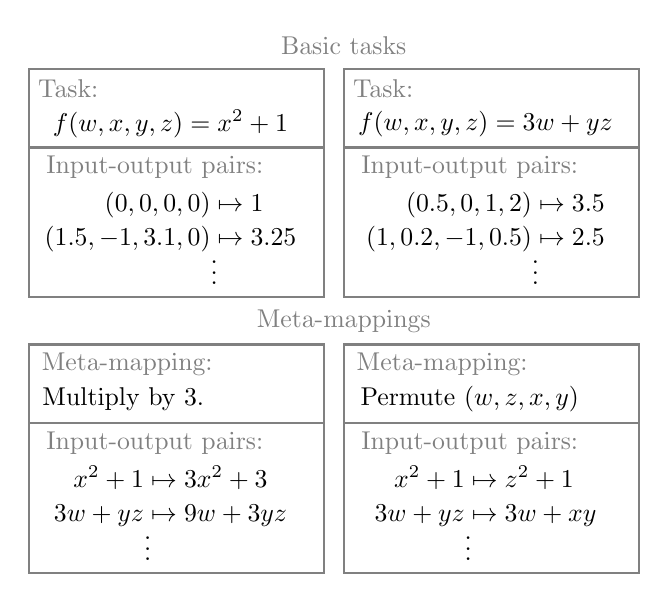
\begin{tikzpicture}[auto, every node/.style={scale=0.93}]
%% Basic
\node[gray] at (0, 3) {Basic tasks};
\draw[boundingbox, draw=gray, fill=white] (-4, 2.7) rectangle (-0.25, -0.2);
\draw[boundingbox, draw=gray, fill=white] (-4, 2.7) rectangle (-0.25, 1.7);
\node[gray] at (-3.5, 2.45) {Task:};
\node[align=center] at (-2.2, 2) {\(f(w,x,y,z) = x^2 + 1\)};
\node[gray] at (-2.4, 1.45) {Input-output pairs:};
\node[align=center] at (-2.2, 0.5) {%
    \(\begin{aligned}
    (0, 0, 0, 0) & \mapsto 1\\[-0.2em] 
    (1.5, -1, 3.1, 0) & \mapsto 3.25\\[-0.75em] 
    & \vdots
    \end{aligned}\)};

\begin{scope}[shift={(4, 0)}]
\draw[boundingbox, draw=gray, fill=white] (-4, 2.7) rectangle (-0.25, -0.2);
\draw[boundingbox, draw=gray, fill=white] (-4, 2.7) rectangle (-0.25, 1.7);
\node[gray] at (-3.5, 2.45) {Task:};
\node[align=center] at (-2.2, 2) {\(f(w,x,y,z) = 3w + yz\)};
\node[gray] at (-2.4, 1.45) {Input-output pairs:};
\node[align=center] at (-2.2, 0.5) {%
    \(\begin{aligned}
    (0.5, 0, 1, 2) & \mapsto 3.5\\[-0.2em] 
    (1, 0.2, -1, 0.5) & \mapsto 2.5\\[-0.75em] 
    & \vdots
    \end{aligned}\)};
\end{scope}

%% meta-mapping
\node[gray] at (0, -0.5) {Meta-mappings};

\begin{scope}[shift={(0, -3.5)}]
\draw[boundingbox, draw=gray, fill=white] (-4, 2.7) rectangle (-0.25, -0.2);
\draw[boundingbox, draw=gray, fill=white] (-4, 2.7) rectangle (-0.25, 1.7);
\node[gray] at (-2.75, 2.45) {Meta-mapping:};
\node[align=center] at (-2.8, 2) {Multiply by 3.};
\node[gray] at (-2.4, 1.45) {Input-output pairs:};
\node[align=center] at (-2.2, 0.5) {%
    \(\begin{aligned}
    x^2 + 1 & \mapsto 3x^2 + 3\\[-0.2em] 
    3w + yz & \mapsto 9w + 3yz\\[-0.75em] 
    & \vdots
    \end{aligned}\)};
\end{scope}

\begin{scope}[shift={(4, -3.5)}]
\draw[boundingbox, draw=gray, fill=white] (-4, 2.7) rectangle (-0.25, -0.2);
\draw[boundingbox, draw=gray, fill=white] (-4, 2.7) rectangle (-0.25, 1.7);
\node[gray] at (-2.75, 2.45) {Meta-mapping:};
\node[align=center] at (-2.4, 2) {Permute \((w, z, x, y)\)};
\node[gray] at (-2.4, 1.45) {Input-output pairs:};
\node[align=center] at (-2.2, 0.5) {%
    \(\begin{aligned}
    x^2 + 1 & \mapsto z^2 + 1\\[-0.2em] 
    3w + yz & \mapsto 3w + xy\\[-0.75em] 
    & \vdots
    \end{aligned}\)};
\end{scope}
\end{tikzpicture}
}}\\
\textbf{Visual concepts (image classification):}
\resizebox{0.9\textwidth}{!}{
\begin{tikzpicture}[auto, scale=0.8, every node/.style={scale=0.8}]
\draw[boundingbox, draw=gray, fill=white] (-9.4, 2.7) rectangle (-0.1, 0);
\node[gray, align=center] at (-4.7, 2.45) {\large Visual concept (basic task)};
\node at (-9, 1.23) {\Huge \color{bgreen} \bigcheckmark};
\draw[decoration={calligraphic brace, amplitude=0.4cm},decorate,line width=1mm] (-8.1, 0.2) -- (-8.1, 2.2);
\node at (-6.6, 1.21) {\includegraphics[width=1.5cm]{figures/categorization/32_yellow_triangle_1.png} \includegraphics[width=1.5cm]{figures/categorization/24_yellow_triangle_1.png}};

\node at (-4.3, 1.21) {\Huge \color{red}\(\bm \times\)};
\draw[decoration={calligraphic brace, amplitude=0.4cm},decorate,line width=1mm] (-3.4, 0.2) -- (-3.4, 2.2);
\node at (-1.9, 1.21) {\includegraphics[width=1.5cm]{figures/categorization/32_yellow_circle_1.png} \includegraphics[width=1.5cm]{figures/categorization/24_blue_triangle_1.png}};

\begin{scope}[shift={(0, -3)}]
\draw[boundingbox, draw=gray, fill=white] (-9.4, 2.7) rectangle (-0.1, 0);
\node[gray, align=center] at (-4.7, 2.45) {\large Transformed concept};
\node at (-9, 1.23) {\Huge \color{bgreen} \bigcheckmark};
\draw[decoration={calligraphic brace, amplitude=0.4cm},decorate,line width=1mm] (-8.1, 0.2) -- (-8.1, 2.2);
\node at (-6.6, 1.21) {\includegraphics[width=1.5cm]{figures/categorization/24_cyan_triangle_0.png} \includegraphics[width=1.5cm]{figures/categorization/32_cyan_triangle_1.png}};

\node at (-4.3, 1.21) {\Huge \color{red}\(\bm \times\)};
\draw[decoration={calligraphic brace, amplitude=0.4cm},decorate,line width=1mm] (-3.4, 0.2) -- (-3.4, 2.2);
\node at (-1.9, 1.21) {\includegraphics[width=1.5cm]{figures/categorization/24_cyan_emptysquare_0.png} \includegraphics[width=1.5cm]{figures/categorization/32_yellow_triangle_1.png}};
\end{scope}

\end{tikzpicture}
}
\end{column}%
\begin{column}{0.5\textwidth}
\textbf{Reinforcement learning:}
\inlineMovie{figures/recording_pusher.mp4}{../../psych/dissertation/4-extending/figures/pusher_0.png}{width=0.9\textwidth, height=0.65\textwidth}
\textbf{Initializing later learning:}
\includegraphics[width=0.9\textwidth]{../../psych/dissertation/5-timescales/figures/polynomial_optimization_curves.png}
\end{column}

\end{columns}

\end{frame}

\begin{frame}{Conclusions}

\begin{itemize}
\item Humans can perform novel tasks without retraining. 
\item I suggest that task transformation offers a useful perspective on this ability. 
\item I propose a computational description of task transformation: \textbf{meta-mapping}.
    \begin{itemize}
        \item And a parsimonious architectural implementation that uses the same networks for basic tasks and meta-mappings. 
    \end{itemize}
\item Meta-mapping performs comparably to humans in a card game task, and outperforms a language based approach.
\item Meta-mapping also performs well across settings ranging from image classification to reinforcement learning, and allows faster, better later learning. 
%\item Earlier paper: \url{https://arxiv.org/abs/1905.09950} and library + all code: \url{https://github.com/lampinen/HoMM}
\end{itemize}
\end{frame}

\begin{frame}[standout]
Thanks, questions?\\[1em]
{\normalsize (Please ``raise hand'' on Zoom, and we will unmute you to ask, or share your question in the chat.)}
\end{frame}

\begin{frame}{Relation to model-based adaptation}
Model-based methods are often framed in part as an approach to flexibility.
\begin{itemize}
\item However, for this to work, these methods generally must have a new reward function handed to them.
\item That is, they're offloading a substantial part of the adaptation problem to another system.
\item Meta-mapping could offer a principled way to adapt a reward predictor, transition models, etc.
\item Thus meta-mapping and model-based planning could be complementary.
\end{itemize}
\end{frame}

\end{document}
